    \documentclass[conference]{IEEEtran}
    \IEEEoverridecommandlockouts
    % The preceding line is only needed to identify funding in the first footnote. If that is unneeded, please comment it out.
    \usepackage{cite}
    \usepackage{amsmath,amssymb,amsfonts}
    \usepackage{algorithmic}
    \usepackage{graphicx}
    \usepackage{textcomp}
    \usepackage{xcolor}
    \usepackage{float}
    \usepackage{listings}


    \def\BibTeX{{\rm B\kern-.05em{\sc i\kern-.025em b}\kern-.08em
        T\kern-.1667em\lower.7ex\hbox{E}\kern-.125emX}}
\begin{document}

\title{Fake News Detection on Social Media\\
    \large DS203:  Programming for Data Science\\
    Course Project
}\\
\author{
    \IEEEauthorblockN{Vinit Awale}
    \IEEEauthorblockA{\textit{Dept. of Electrical Engg.} \\
        \textit{Indian Institute of Technology, Bombay}\\
        Mumbai, India \\
        18D070067@iitb.ac.in}
}

\maketitle

\begin{abstract}
% In the present times, malware attacks are one of the rising concerns regarding the security of users' data. In this project we attempt to use Machine learning techniques to determine the probability of a machine to be affected by malware. Comparison of the the Machine Learning Models Logistic Regression, KNN, Random Forest Classifier and LGBM for making predictions has been done. Since the dataset is quite large (more than 8GB!), the problem becomes a very high dimensionality problem. Hence, data preprocessing and feature engineering becomes very important in handling the given dataset and this has been done in the implementation. A prediction accuracy of 63.15 percent was obtained in making predictions.

In the present times, Social Media has become an indispensable part of our life. The ubiquitousness of smartphones enables people to announce an emergency they’re observing in real-time. This is a great opportunity for people to share their news and information with their friends and family. However, the news and information that is shared on social media is not always accurate. This is where the concept of Fake News comes into play. Fake News is a news that is created by a person or organization that is not the original source of the news. This is a type of misinformation that is used to spread misinformation. In this project, we have used Machine Learning techniques to determine the probability of whether a given news is fake or not.

\begin{IEEEkeywords}
    \key{Fake News Detection}, \key{Machine Learning}, \key{Social Media}, \key{Data Science}
\end{IEEEkeywords}

\section{Introduction}
In the present times, malware attacks are one of the rising concerns regarding the security of users' data. The malware industry is a well-organized, well-funded market dedicated to evading traditional security measures. Once a computer is infected by malware, criminals can hurt consumers and enterprises in many ways.According to the survey conducted by NetMarketShare, $87\%$ of the Operating Systems Market Share is ruled by Microsoft Windows. Hence, this problem statement was uploaded by \textit{Microsoft, Windows Defender ATP Research, Northeastern University College of Computer and Information Science and Georgia Tech. Institute} on Kaggle competitions.\\
In this project we attempt to use Machine learning techniques to determine the probability of a machine to be affected by malware.The challenge one faces while solving this problem is obtaining the dataset with appropriate features for determining the probability of a malware attack. However, Microsoft has provided an unprecedented malware dataset which resolves this problem for us. However, the dataset is quite large and the problem becomes a very high dimensionality problem owing to the large number of features included in the data set. As a result, the data preprocessing and feature engineering becomes very important in handling the given dataset.\\
Summarising the results of our project:
\begin{itemize}
    \item We compared the Machine Learning Models Logistic Regression, KNN, Random Forest Classifier and LGBM for making predictions.
    \item We obtained a prediction accuracy of $63.15 \%$ in making predictions
    \item Concluded that the feature AVSig Version (which is the version of the database of signatures of the anti virus) is the most important feature in determining if the machine is likely to face a malware attack
\end{itemize}

\section{Background and Previous Work}
Since the dataset is quite large and the problem becomes a very high dimensionality problem data preprocessing and feature engineering becomes very important in handling the given dataset. Hence, apart from knowing basic ML having knowledge about the Computer Architecture and Cyber Security can help in determining the features which contribute more towards making the final prediction. Previously, various competitors have attempted  to get the highest possible accuracy using various ML models. In this project, we attempt to compare the various models taught in the course and to compare them with the benchmark scores obtained by the other competitors.

\section{Methodology}
For this project, we have used the dataset from the Kaggle competition where this problem statement was posted. The dataset has two files, train.csv and test.csv .
\begin{itemize}
    \item Train.csv : This data file has 8921483 entries and 83 columns for each entry.
          These columns also include 'HasDetections' which indicates whether the given machine has been affected by malware.
    \item Test.csv : This data file has 7853253 entries. It contains 82 columns for each entry since it doesn't include the 'HasDetections' columns as compared to the Train.csv.
\end{itemize}

\section{Experiments and Results}
\subsection{Loading the Dataset}
We first loaded the dataset and had a look at the first few entries of the dataset. The dataset has two files, train.csv and test.csv. The entries in train.csv are as follows:
\begin{figure}[H]
    \centering
    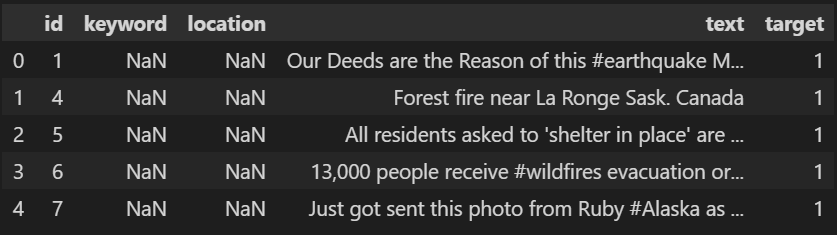
\includegraphics[width=0.4\textwidth]{Results/train.png}
    \caption{Entries in the train.csv file}
\end{figure}
The entries in test.csv are as follows:
\begin{figure}[H]
    \centering
    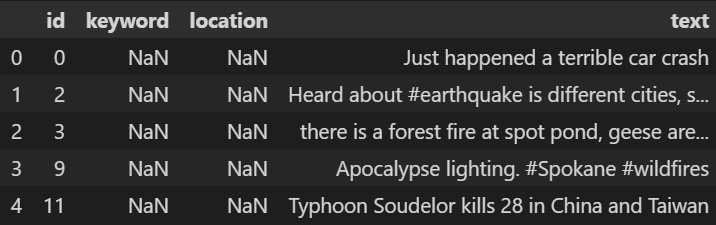
\includegraphics[width=0.4\textwidth]{Results/test.png}
    \caption{Entries in the test.csv file}
\end{figure}

Also we observed that there are 7613 rows and 7 columns in train dataset and there are 3263 rows and 4 columns in test dataset.



\subsection{Exploratory Data Analysis}
After loading the dataset, we have performed exploratory data analysis on the data. We have performed the following:
\subsubsection{Target Value Distribution}
For our case the target value is binary i.e. 0 or 1. In other words, a given tweet is either fake or not. We first have a look at the distribution of the target values in the dataset. For this,we have made a pie chart of the target values.

\begin{figure}[H]
    \centering
    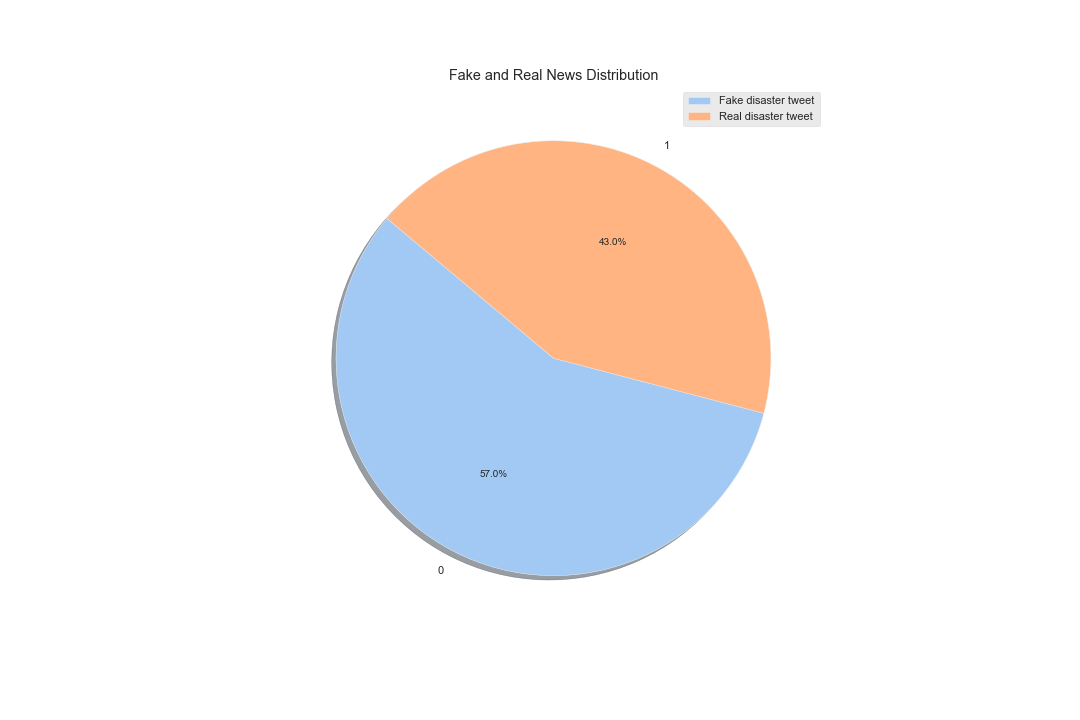
\includegraphics[width=0.3\textwidth]{Results/Fake_News_Prediction_Pie_Chart.png}
    \caption{Distribution of the target values in the dataset}
\end{figure}
Hence we observed that the dataset is skewed towards the Fake News. 57\% of the data is Fake News.

\subsubsection{Exploring Locations of the Tweets}
After looking at the distribution of the target values, we have decided to explore the location of the tweets. We have made a bar chart of the locations of the tweets for the top 15 locations.
\begin{figure}[H]
    \centering
    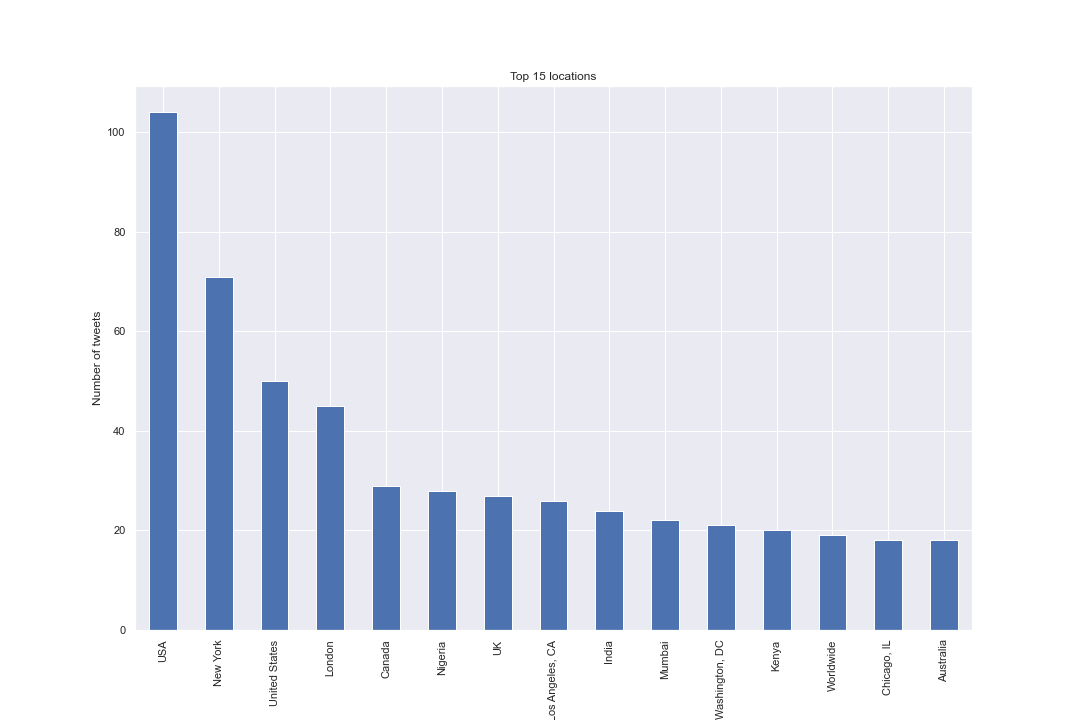
\includegraphics[width=0.5\textwidth]{Results/Location_Bar_Plot.png}
    \caption{Bar chart of the top 15 locations of the tweets}
\end{figure}

From the above bar chart, we can observe that the location of the tweets are mostly in the United States. It is then followed by New-York and London.

Further to get a better visualization of the location of the tweets, we have made a map of the locations of the tweets.
\begin{figure}[H]
    \centering
    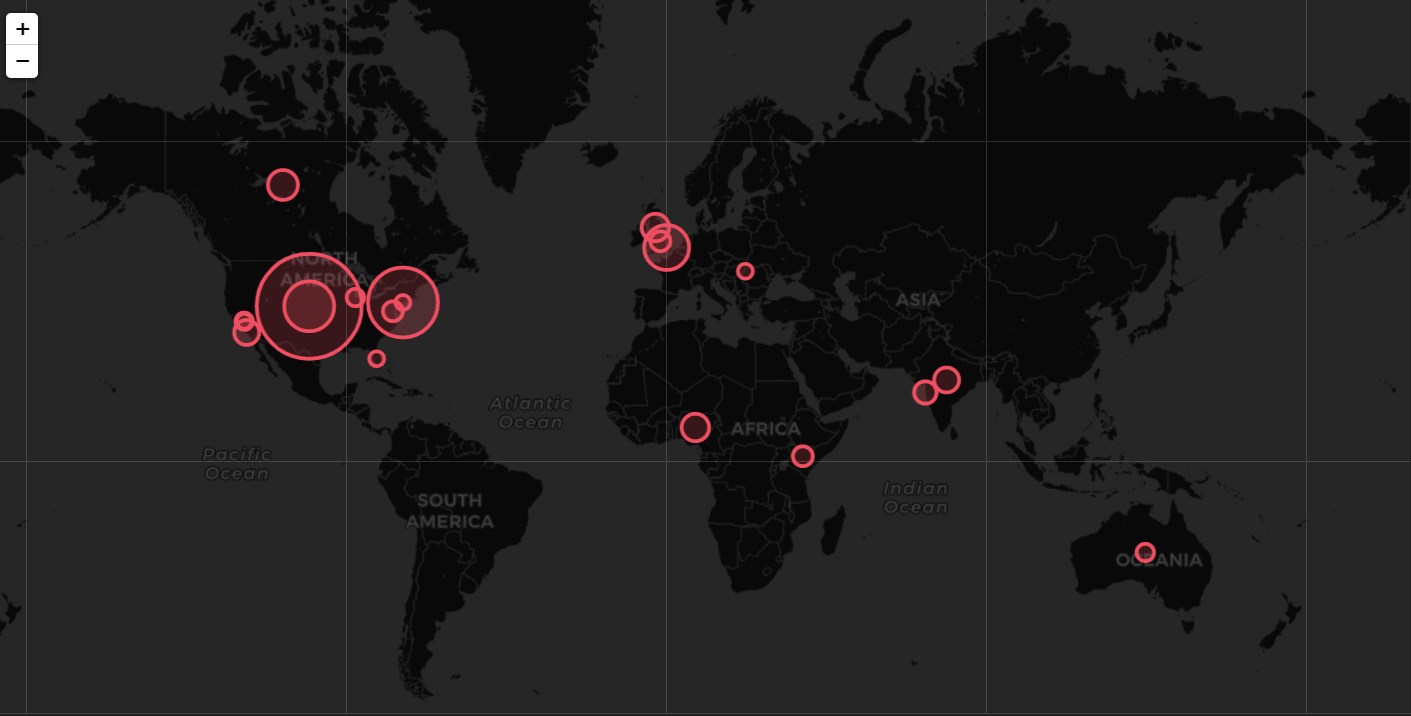
\includegraphics[width=0.5\textwidth]{Results/Tweets_location_on_map.png}
    \caption{Map of the locations of the tweets}
\end{figure}

\subsubsection{Distribution of the Real and Fake Tweets based on the location}
We have made a bar chart of the distribution of the tweets based on the location.
\begin{figure}[H]
    \centering
    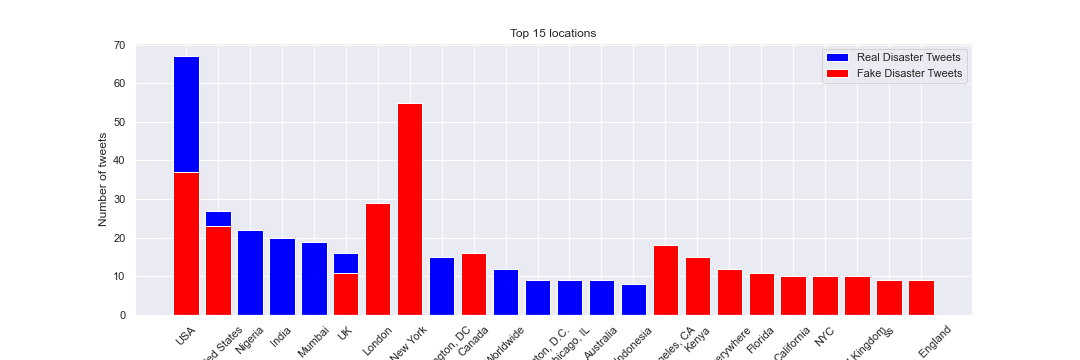
\includegraphics[width=0.5\textwidth]{Results/Location_Distribution_Bar_Plot.png}
    \caption{Bar chart of the distribution of the tweets based on the location}
\end{figure}

From the above bar chart we observe that number of fake news from location USA is more than the number of real news from location USA. Also,for other locations such as India all the tweets are real news.

\subsection{Distribution of word count in Real and Fake Tweets}
We have made a bar chart of the distribution of the word count in the tweets.
\begin{figure}[H]
    \centering
    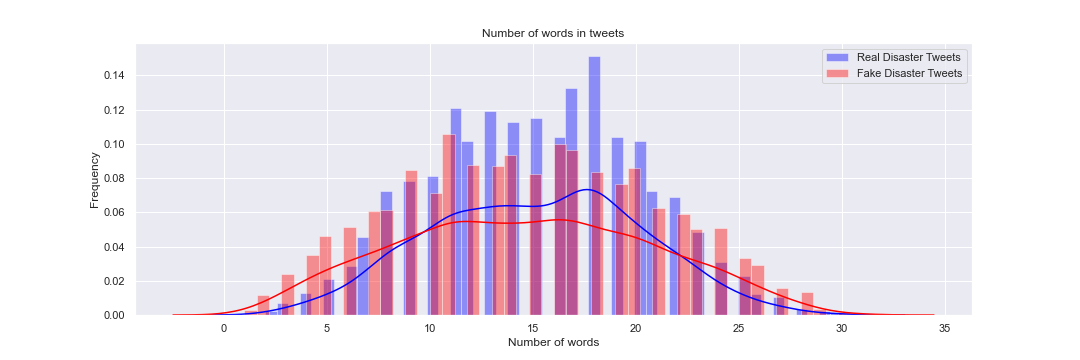
\includegraphics[width=0.5\textwidth]{Results/Number_of_words_in_Tweets_Distribution_Bar_Plot.png}
    \caption{Bar chart of the distribution of the word count in the tweets}
\end{figure}

From the above plot we can observe that the distribution of fake disasters is skewed towards the left side of the plot. This is because the word count of the fake news is less than the word count of the real news.


\subsection{Distribution of character count in Real and Fake Tweets}
We have made a bar chart of the distribution of the character count in the tweets.
\begin{figure}[H]
    \centering
    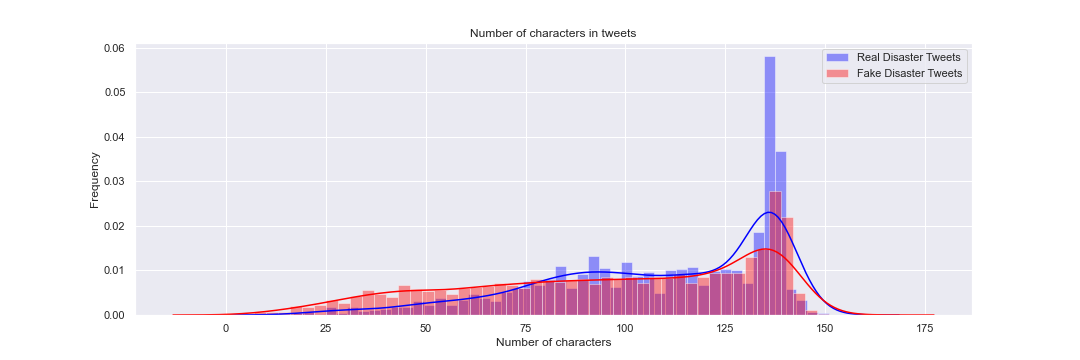
\includegraphics[width=0.5\textwidth]{Results/Number_of_characters_in_Tweets_Distribution_Bar_Plot.png}
    \caption{Bar chart of the distribution of the character count in the tweets}
\end{figure}

From the above plot we can see that the distribution of both real and fake tweets is similar. Hence, we can conclude that the character count of the tweets is similar.

\subsection{Data Cleaning and Tokenization}
After EDA, we started with the data cleaning process. Here, our objective was to make the data more consistent and clean so that we can use it for our analysis and make predictions using a machine learning model. The tokenization of tweets can be done using Keras' Tokenizer. Before that we perform some basic cleaning of the data.

We removed the following from the tweets dataset:
\begin{itemize}
    \item Punctuation
    \item Stop words
    \item Non-alphanumeric characters
    \item URLs
    \item HTML tags
    \item Emojis
\end{itemize}

The punctuation to the sentence adds up noise that brings ambiguity while training the model. English is one of the most common languages, especially in the world of social media. For instance, "a," "our," "for," "in," etc. are in the set of most commonly used words. Removing these words helps the model to consider only key features. These words also don't carry much information. By eliminating these words, we can improve the accuracy of the model.
The common stop words in English language have been taken from the NLTK library. These are shown below:
\begin{figure}[H]
    \centering
    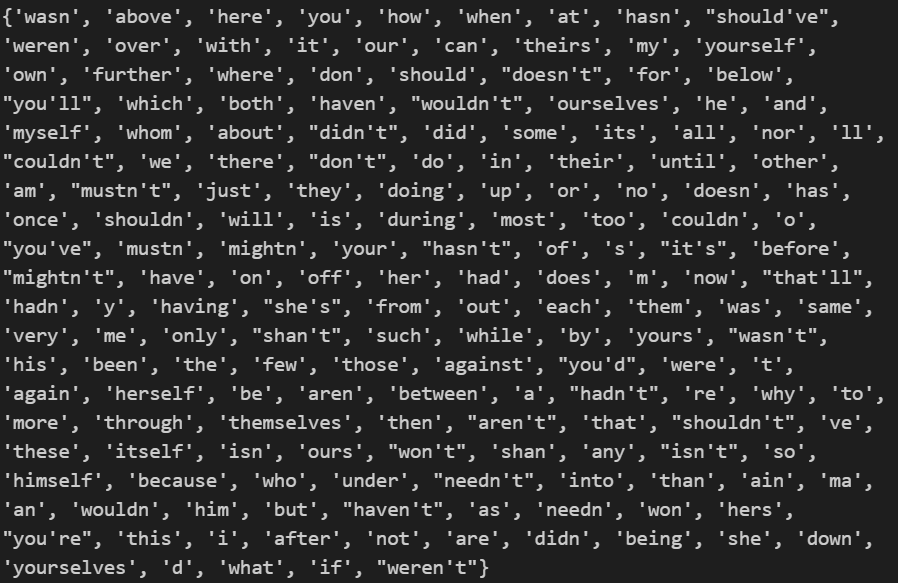
\includegraphics[width=0.5\textwidth]{Results/Stop_words.png}
    \caption{Common stop words in English language}
\end{figure}

Also, we removed the URLs, HTML tags and Emojis from the tweets. This helps the model to consider only the important features. The dataset with just the cleaned tweets (without including any meta-data) is as follows:

\subsubsection{Expanding the contractions in the Tweets}
Contractions are used to describe a word or phrase in a sentence. For example, I'm, I've, I'll, I'd, I'll, etc. are contractions. We have expanded the contractions in the tweets. This will help in reducing the noise in the dataset. We considered different contractions mentioned in the link \url{https://stackoverflow.com/questions/19790188/expanding-english-language-contractions-in-python } \\
An example of the expanded contractions used are:
\begin{itemize}
\item "aren't": "are not / am not"
\item "can't": "cannot"
\item "can't've": "cannot have"
\item "'cause": "because"
\item "could've": "could have"
\item "couldn't": "could not"
\item "couldn't've": "could not have"
\item "didn't": "did not"
\item"doesn't": "does not"


\subsection{Test-Train Split}
Since the dataset is quite large we take a relatively small portion of the dataset to test and train the model. We have taken 10000 entries to lower the computational time. Then we have split this data into training and testing (For validation) dataset.

\subsection{Training the model}
For making predictions we have used the SciKit Learn implementaions of the models\footnote{The implementation code has been included in the Jupyter notebook. The notebook link has been mentioned in references.}
\begin{itemize}
    \item Logistic Regression
    \item KNN
    \item Random Forest Classifier
\end{itemize}

We then compared the accuracy of the three models used.
\begin{figure}[H]
    \centering
    \includegraphics[width=\linewidth]{11.png}
\end{figure}


\subsection{Hyperparameter Tuning}
\subsubsection{KNN}
We varied the value of the hyperparamter K from 1 to 30 and observed the accuracy on the testing data.
\begin{figure}[H]
    \centering
    \includegraphics[width=\linewidth]{12.png}
\end{figure}

We can see that we get the highest accuracy on test data for K=9. The obtained accuracy is as follows.
\begin{figure}[H]
    \centering
    \includegraphics[width=\linewidth]{13.png}
\end{figure}

From the obtained results we can easily see that KNN model is overfitting and the reason is that because of excessive number of data points.

\subsubsection{Logistic Regression}
We used Randomized Search CV for varying the following hyperparameters of Logistic Regression.
\begin{figure}[H]
    \centering
    \includegraphics[width=\linewidth]{14.png}
\end{figure}
The best hyperparameters obtained are
\begin{figure}[H]
    \centering
    \includegraphics[width=\linewidth]{15.png}
\end{figure}

For these hyperparameters we get an accuracy of $52.25 \%$

\subsubsection{Random Forest Classifier}
We used Randomized Search CV for varying the following hyperparameters of Random Forest Classifier.
\begin{figure}[H]
    \centering
    \includegraphics[width=\linewidth]{16.png}
\end{figure}
The best hyperparameters obtained are
\begin{figure}[H]
    \centering
    \includegraphics[width=\linewidth]{17.png}
\end{figure}

For these hyperparameters we get an accuracy of $62.80 \%$

\subsection{Feature Engineering and Training Model with important Features}

We obtained the importance of the various features. The plot of it is as follows.
\begin{figure}[H]
    \centering
    \includegraphics[width=\linewidth]{18.png}
\end{figure}

We decided to keep only the features with a score greater than 0.01. Using these features we again trained a Random Forest Classifier using the best hyperparameters as obtained earlier.
\begin{figure}[H]
    \centering
    \includegraphics[width=\linewidth]{19.png}
\end{figure}

Hence, by feature engineering our accuracy on test data went up from $62.80 \%$ to $63.15 \%$.

\subsection{Correlation among the features}
Finally we plotted a dendogram to obtain the correlation among the various features.
\begin{figure}[H]
    \centering
    \includegraphics[width=\linewidth]{20.png}
\end{figure}

\subsection{Using LGBM (Light Gradient Boosting Machine) model for Predictions}
We used the data under consideration after feature engineering to train the LGBM model. We used Light GBM  because it is a fast, distributed, high-performance gradient boosting framework based on decision tree algorithm, used for ranking, classification and many other machine learning tasks.Since it is based on decision tree algorithms, it splits the tree leaf wise with the best fit whereas other boosting algorithms split the tree depth wise or level wise rather than leaf-wise. So when growing on the same leaf in Light GBM, the leaf-wise algorithm can reduce more loss than the level-wise algorithm and hence results in much better accuracy which can rarely be achieved by any of the existing boosting algorithms. \\
Finally we obtained a prediction accuracy of $\mathbf{60.55 \%}$ at a runtime of $468 \mu s$.


\section{Conclusions}
\begin{itemize}
    \item Whenever we choose different machine learning models for carrying out training and testing, for similar model complexity there is a tradeoff. Some models offer higher prediction accuracy but consume higher computuational resources whereas some models give lower prediction accuracy but at a much lower time.
    \item This tradeoff can also be observed in the project. The comparision of run-time and prediction accuracy of the models under comparison is as below.
          \begin{table}[H]
              \centering
              \begin{tabular}{|c|c|c|}
                  \hline
                  Model               & Runtime       & Prediction Accuracy \\ \hline
                  Logistic Regression & $72.3 \mu s $ & $52.25 \%$          \\
                  KNN                 & $276 \mu s$   & $53.75 \%$          \\
                  Random Forest       & $2.83 s$      & $63.15 \%$          \\
                  LGBM                & $468 \mu s$   & $60.55 \%$          \\
                  \hline
              \end{tabular}
              \caption{Comparison of runtime and prediction accuracy for the algorithm}
          \end{table}
    \item We can easily see that LGBM model comparatively works very well on this dataset. It takes very less runtime compared to Random Forest, however its prediction accuracy is comparable to that of Random Forest.
    \item We obtained a prediction accuracy of $63.15 \%$ in making predictions.
    \item Concluded that the feature AVSig Version (which is the version of the database of signatures of the anti virus) is the most important feature in determining if the machine is likely to face a malware attack.
\end{itemize}


\section{Limitations}
\begin{itemize}
    \item Firstly, due to limited computational resources we worked on a very small sample from the dataset. Hence, we can expect the prediction accuracy to be higher when we use the complete dataset with all the models. The highest prediction accuracy obtained in the competition was roughly $69 \%$ using LGBM, however, they used more number of samples from the data set and hence higher computational time.
    \item Due to time constraints of the project, we could not compare the Neural Networks model. However, we did expect LGBM to work better on the given dataset and hence we skipped Neural Networks and directly moved on to LGBM.
    \item With some prior knowledge of Operating Systems and Computer Architecture, we could have dropped some of the less important features by mere observation, which couldn't be done in this project.
\end{itemize}


\section{Work Contribution}
\begin{table}[H]
    \centering
    \begin{tabular}{|c|c|c|}
        \hline
        Task                              & Aniket     & Vinit     \\ \hline
        Project Conception                & 2.5 hours  & 2.5 hours \\
        Data Collection                   & -          & 1 hour    \\
        Coding                            & 10.5 hours & 4.5 hours \\
        Report                            & 4.5 hours  & 9.5 hours \\
        Getting introduced LGBM Algorithm & 0.5 hours  & 0.5 hours \\
        Slides and Video Presentation     & 2 hours    & 2 hours   \\
        \hline
    \end{tabular}
\end{table}
\begin{thebibliography}{00}
    \bibitem{b1} https://colab.research.google.com/drive/1Q7pwCLvbUV4G1kgtcy8RWJveq2-XkCYE?usp=sharing
    \bibitem{b2} https://www.kaggle.com/c/microsoft-malware-prediction/data?select=test.csv
    \bibitem{b3} https://lightgbm.readthedocs.io/en/latest
\end{thebibliography}
\end{document}
